\newpage
\section{Contribution}
Dans cette section, nous présentons la contribution faite dans le cadre du stage.
Nous commençons par lister le cahier des charges du stage.
Ensuite, nous allons parler de la contribution et expliquer les différents choix d'implémentation.


\subsection{Cahier des charges}
Dans cette section, nous allons définir le cahier des charges du projet.

\subsubsection{JSON}
La carte d’identité de la machine virtuelle est exprimée sous la forme d’un JSON contenant les empreintes des deux éléments permettant de caractériser une machine virtuelle afin d’assurer la propriété d’intégrité.\cite{cdc}
Elle contient trois éléments principaux :
\begin{description}
    \item[uuid]  L’identifiant alphanumérique de la machine virtuelle, chaque machine
    virtuelle disposant d’un identifiant unique.
    \item[type] Le type de migration effectué :
    \begin{description}
        \item[cold] Migration à froid de la machine virtuelle. La machine virtuelle est
        éteinte/suspendue et son image disque est migrée entre les deux fournisseurs.
        \item[lan] Migration à chaud avec disque dur partagé. La machine virtuelle
        est migrée sans interruption de service. Le disque dur est partagé
        (NFS, iSCSI...) entre la machine virtuelle source et destination, seule
        la mémoire est donc activement migrée.
        \item[wan] Le disque dur n'est pas partagé entre la machine virtuelle source et destination, ça migration est donc nécessaire ainsi que la mémoire.
    \end{description} 
    \item[fingerprints] Section contenant les empreintes devant être utilisées pour caractériser la VM. Elle contient deux sous-sections:
    \begin{description}
        \item[memory] Cette sous-section contient l’empreinte permettant d’identifier
        les données mémoire.
        
        \item[disk] Cette sous-section contient l’empreinte permettant d’identifier les
        données disques.

        Une empreinte est identifiée par un dictionnaire contenant deux couples de clef valeur :
        \item[algorithm] L’algorithme utilisé pour calculer l’empreinte.
        \item[hash]  L’empreinte effective du périphérique.
        Les deux sections memory et disk ne sont pas obligatoirement présentes selon le type de migration effectué :

        \begin{figure}[H]
            \centering
            \begin{tabular}{|c | c | c | c |} 
                \hline
                Présence & cold & lan & wan \\ 
                \hline
                memory & NON & OUI & OUI \\ \hline
                disk & OUI & NON & OUI \\ \hline
            \end{tabular}
            \caption{Tableau de types de migration}
        \end{figure}

    \end{description}

    \item[hypervisor] Une description de l’hyperviseur source et de la configuration nécessaire pour accueillir la machine virtuelle migrée.
    Elle contient trois sous-sections :

    \begin{description}
        \item[name] Le nom de l’hyperviseur source.
        \item[version] La version de l’hyperviseur source.
        \item[configuration] Une description de la configuration nécessaire à la migration. 
        Cette description varie selon les hyperviseurs et n’est donc pas normalisée.
    \end{description} 

\end{description}

Voici un exemple de la sortie souhaité:
\begin{lstlisting}[language=json,caption={Exemple de carte d'identité de migration},captionpos=b]
{
    "uuid": "oUXbdAEtCStygyfdzytRYfdy",
    "migration_type": "wan",
    "fingerprints": {
        "memory": {
            "algorithm": "sha256",
            "hash":"2b5326bed38bf8b344f4faddaaa80e1f6428   b844b384251e431ca1353248123b"
        },
        "disk": {
            "algorithm": "sha256",
            "hash":"e45ba2e4318f64ad7fedbcf666c481a34eba   12f4599b31dc21eac3242cc7a12a"
        },
    },
    "hypervisor": {
        "name": "kvm",
        "version": "5.2.50",
        "configuration": {
            "memory": 1024,
            "vcpus": 2,
            "disk": {
                "driver": {
                    "name": "qemu",
                    "bus": "virtio",
                    "file": "/var/images/vm.qcow2",
                    "if": "virtio"
                }
            }
        }
    }
}
\end{lstlisting}

\subsection{Solution}
Dans cette section, nous allons parler des différentes contributions du projet et du choix de nos implémentations.

\subsubsection{Calcul de l'empreinte de la machine virtuelle}
En vue de sécuriser l'intégrité des données échangées, la réalisation d'une empreinte de machine virtuelle met en exergue des problématiques de performances.
En effet, afin de minimiser les latences de migration, il est nécessaire de calculer le plus rapidement possible l’empreinte d’une machine virtuelle.
Celle-ci peut potentiellement manipuler un volume de données conséquent dont les données changent constamment.
Or, les fonctions de hash traditionnelles devant être exécutées lors de l'arrêt de la machine source engendrent des temps de calcul et des latences additionnelles qui sont prohibitives.\cite{usecase}

Les solutions de calcul de hash en mode flux permettent aussi de répartir le temps de calcul de l'empreinte pendant que la machine virtuelle est en cours d’exécution (Total time) et ainsi éviter de faire la totalité du calcul lors de la phase de downtime (l'arrêt de la machine source).

Nous avons choisi l'algorithme SHA-1 pour notre implémentation. 
Celui-ci propose une fiabilité suffisante et la vitesse de hash est supérieur à MD5 et SHA-256.

\subsubsection{Différentes approches de la résolution du problème}
Lors du processus de résolution de la problématique, il a fallu se confronter à l'analyse de la pile d'appels des fonctions pour transformer les données (Page de RAM, bloc de disque, état des périphériques ...) en un flux binaire qui serra transmis lors de la migration.
Il a fallu chercher le meilleur endroit dans cette pile d'appels de fonction pour faire le calcul du hash.\cite{usecase}

Ce graphique propose une vue simpliste des différentes portions ou le calcul de l'empreinte peut se faire.
\begin{figure}[H]
\centering
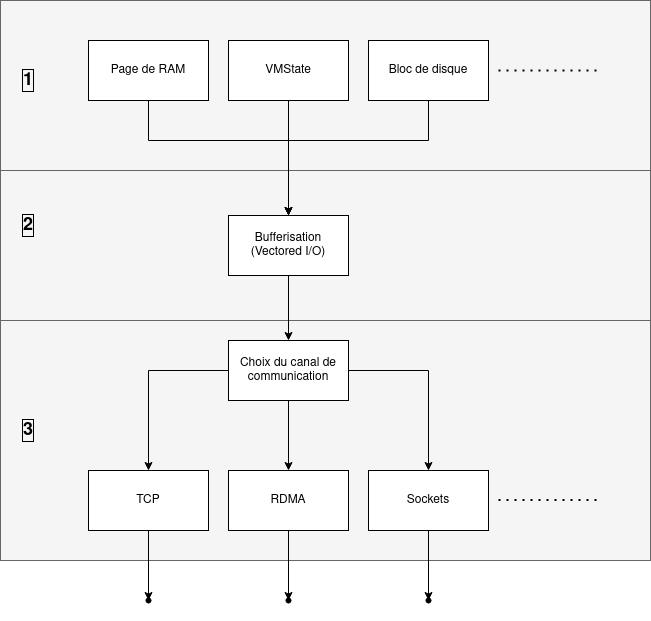
\includegraphics[scale=0.5]{include/placement.png}
\caption{Représentation graphique des différentes approches}
\end{figure}


\begin{description}
    \item[Partie 1] dans ce niveau sont envoyées les données (sous forme d'octet ou de bloc de données) de l'état des différents périphériques.
    
    Les avantages de faire le calcul de hash dans ce niveau sont :
    \begin{enumerate}
    \item Connaissance du type de données envoyé (device, ram, disque).
    \item Les données des headers de section ne sont pas inclues dans le calcul de hash, impliquant moins de temps CPU.
    \end{enumerate}
    Les inconvénients de faire le calcul de hash dans ce niveau sont :
    \begin{enumerate}
    \item Non-générique.
    \item Il est nécessaire de rajouter du code dans toutes fonctions qui envoient des données lors de la migration (chaque device, ram, disque).
    \item De nouveaux périphériques peuvent être ajoutés, impliquant du code supplémentaire pour le calcul de l'empreinte.
    \end{enumerate}
    
    \item[Partie 2] dans ce niveau les données transmises sont mises dans des vecteurs de tampons (iovec).
    Cela permet de travailler avec des blocs de données non-contigus, c'est-à-dire que les différents blocs de données peuvent être alloués séparément, pour être à la fin écrit dans un seul flux de donnée.
    
    Les avantages de faire le calcul de hash dans ce niveau sont :
    \begin{enumerate}
    \item Générique.
    \item Facile, peu de code à rajouter.
    \end{enumerate}
    Les inconvénients de faire le calcul de hash dans ce niveau sont :
    \begin{enumerate}
    \item Connaissance limitée du type de données envoyé (device, ram, disque).
    \item Les données des headers de section sont incluses dans le calcul de l'empreinte.
    \end{enumerate}
    \item[Partie 3] dans ce niveau les données sont aiguillés vers le bon protocole de transport, et les routines associées sont appelées pour transférer le flux de donnée.
    
    Les inconvénients de faire le calcul de hash dans ce niveau sont :
    \begin{enumerate}
    \item Les routines de tous les protocoles doivent être modifier pour inclure le calcul de l'empreinte.
    \item Les données étant bufferisées, il est n'est pas possible de distinguer le type des données (Disque, RAM) qui transite sans faire du calcul CPU supplémentaire pour chercher les différents headers de section.
    \end{enumerate}
    
    \end{description}
    
    \subsubsubsection{Approche retenue}
    L'approche implémentée lors du stage est celle de niveau 2.
    
    \begin{figure}[H]
    \centering
    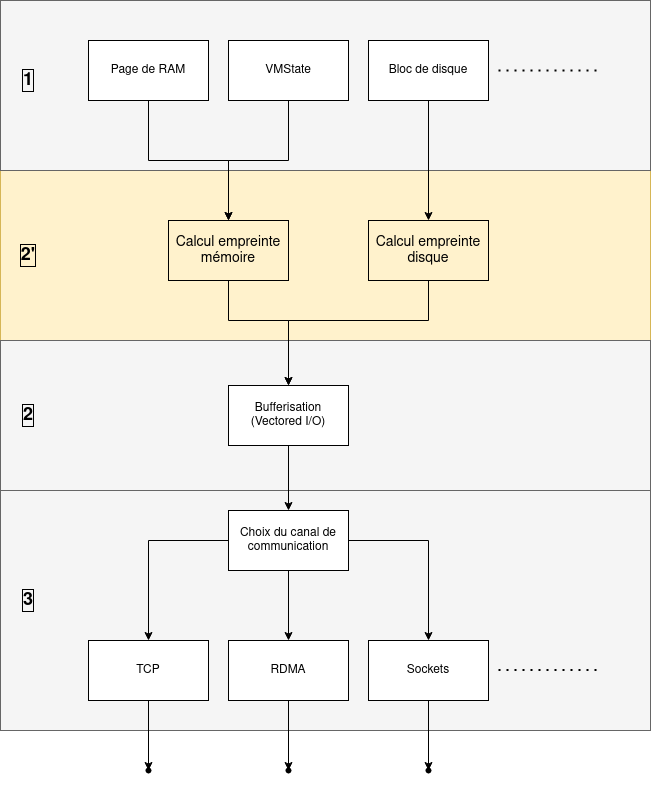
\includegraphics[scale=0.5]{include/implem.png}
    \caption{Représentation graphique de approche retenue}
    \end{figure}
    
    L’implémentation consiste à hasher toutes les données qui sont envoyées par les différents devices (RAM, Disque, CPU ...). Il sera donc nécessaire de reconnaître les différents devices pour générer des hash différents : un pour la RAM et les différents périphérique et un autre dédié au disque.    
    
    Les différentes informations sur l'empreinte générée sont stockées dans une structure de donnée, déjà existante, \texttt{QEMUFile} qui sert à identifier le flux de migration (que ce soit de type rdma, fd, tcp ...).
    
    Après notre implémentation, la structure de donnée ressemble à :

\begin{lstlisting}[caption={Structure de donnée QEMUFile},captionpos=b]
    typedef struct QEMUFile {
        const QEMUFileOps *ops;
        const QEMUFileHooks *hooks;
        void *opaque;
    
        int64_t bytes_xfer;
        int64_t xfer_limit;
    
        int64_t pos; /* start of buffer when writing, end of buffer
                        when reading */
        int buf_index;
        int buf_size; /* 0 when writing */
        uint8_t buf[IO_BUF_SIZE];
    
        DECLARE_BITMAP(may_free, MAX_IOV_SIZE);
        struct iovec iov[MAX_IOV_SIZE];
        unsigned int iovcnt;
    
        int last_error;
        Error *last_error_obj;
        /* has the file has been shutdown */
        bool shutdown;
    
        //Fingerprint patch
        int is_wan;
        SHA_CTX hash_context;
        SHA_CTX hash_disk_context;
        QJSON *json_fingerprint;
        char *fingerprint_path;
        QemuUUID uuid;
    
    } QEMUFile;
\end{lstlisting}

Les différents ajouts sont :
\begin{description}
    \item[is\_wan] Permet de savoir si la migration de la machine virtuelle doit aussi procéder à la migration du disque.
    \item[hash\_context] Permet de calculer le hash de la mémoire et des différents périphériques.
    \item[hash\_disk\_context] Comme précédemment, ce champ permet de calculer le hash disque si \texttt{is\_wan} est à 1.
    \item[json\_fingerprint] Contient le contenu du fichier json qui serra généré à la fin de la migration et qui va contenir les différentes informations de l'empreinte de la machine virtuelle.
    \item[fingerprint\_path] Contient le chemin vers le fichier json en question.
    \item[uuid] Identifiant unique de la machine virtuelle.
\end{description}

Lors du lancement de la migration, ces différents champs sont initialisés.

\begin{lstlisting}[caption={Phase d'initialisation de la structure de donnée},captionpos=b]
    SHA1_Init(&(f->hash_context));
    if(f->is_wan)
        SHA1_Init(&(f->hash_disk_context));
    f->json_fingerprint = qjson_new();
\end{lstlisting}

Par la suite, chaque octet qui est transféré sur le réseau doit inévitablement faire évoluer (mettre à jour) l'empreinte de la machine virtuelle.
Vu que notre choix d'implémentation est au niveau 2, cela va nous permettre d'écrire moins de code (code générique) et ainsi être plus flexible lors des mises à jour de QEMU.

\begin{lstlisting}[caption={Mise à jour de l'empreinte de la machine virtuelle},captionpos=b]
SHA1_Update(&(f->hash_context), buffer, size);
\end{lstlisting}

À la fin de la migration (phase d'arrêt), il va falloir générer l'empreinte finale de la machine virtuelle et créer les fichiers JSON pour être sur de l'intégrité de la migration.

\begin{lstlisting}[caption={Action lors de la fin de la migration},captionpos=b]  
void fingerprint_process(QEMUFile *f) {
    unsigned char c[SHA_DIGEST_LENGTH];
    unsigned char hash[SHA_DIGEST_LENGTH*2];
    char *uuid = qemu_uuid_unparse_strdup(&(f->uuid));
    json_prop_str(f->json_fingerprint, "uuid", uuid);
    
    if (f->is_wan)
        json_prop_str(f->json_fingerprint, "migration_type", "wan");
    else
        json_prop_str(f->json_fingerprint, "migration_type", "lan");


    json_start_object(f->json_fingerprint, "fingerprints");
    
    SHA1_Final(c, &(f->hash_context));
    for (int i=0; i < SHA_DIGEST_LENGTH; i++) {
        sprintf((char*)&(hash[i*2]), "%02x", c[i]);
    }
    json_start_object(f->json_fingerprint, "memory");
    json_prop_str(f->json_fingerprint, "algorithm", "sha256");
    json_prop_str(f->json_fingerprint, "hash", (const char *)hash);
    json_end_object(f->json_fingerprint);

    if (f->is_wan) {
        SHA1_Final(c, &(f->hash_disk_context));
        for (int i=0; i < SHA_DIGEST_LENGTH; i++) {
            sprintf((char*)&(hash[i*2]), "%02x", c[i]);
        }
        json_start_object(f->json_fingerprint, "disk");
        json_prop_str(f->json_fingerprint, "algorithm", "sha256");
        json_prop_str(f->json_fingerprint, "hash", (const char *)hash);
        json_end_object(f->json_fingerprint);
    }

    json_end_object(f->json_fingerprint);

    qjson_finish(f->json_fingerprint);
    
    if(f->fingerprint_path) {
        FILE * fp;
        fp = fopen (f->fingerprint_path, "w+");
        fprintf(fp, "%s\n", qjson_get_str(f->json_fingerprint));        
        fclose(fp);
    }
}
\end{lstlisting}

Il faut prendre en compte que ces trois phases sont à la fois appliquées sur la machine source ainsi que la machine destination.


\subsubsubsection{Démarche de résolution de la problématique}
L'une des étapes les plus importante du stage a été d'analyser le code de la migration de QEMU ainsi que des différentes structures des données et leurs interactions avec l'intégrité du système.
En effet, il a fallu suivre l'acheminement des données de leur envoi depuis différents devices jusqu'à leur réception par la machine virtuelle destination.
Afin de vérifier que les données envoyées (source) et reçues (destination) soient équivalentes.

Dans un premier temps, nous avons récupéré chaque donnée envoyée par les périphériques à travers des sondes.
Ces sondes ont pour but de récupérer et écrire chaque octet sur un fichier.
À la fin de la migration, nous aurons deux fichiers : l'un qui représente les données envoyées par la machine virtuelle source et l'autre les données reçues par la machine virtuelle destination.
Le but final est de comparer les deux fichiers. 
Si aucune altération n'est survenue durant la migration, le contenu des deux fichiers seront équivalents générant alors deux hash identiques, résolvant notre problématique.
En vérifiant les hashs avec des outils de comparaison de code binaire (Hexcompare), nous nous sommes aperçu que quelques centaines de méga-octets de données était différent et changeait d'une migration à une autre.
Cela impliquait que les deux empreintes des VMs n'étaient pas équivalentes or la migration s'était déroulé sans altération de l'intégrité des données.
\begin{figure}[H]
\centering
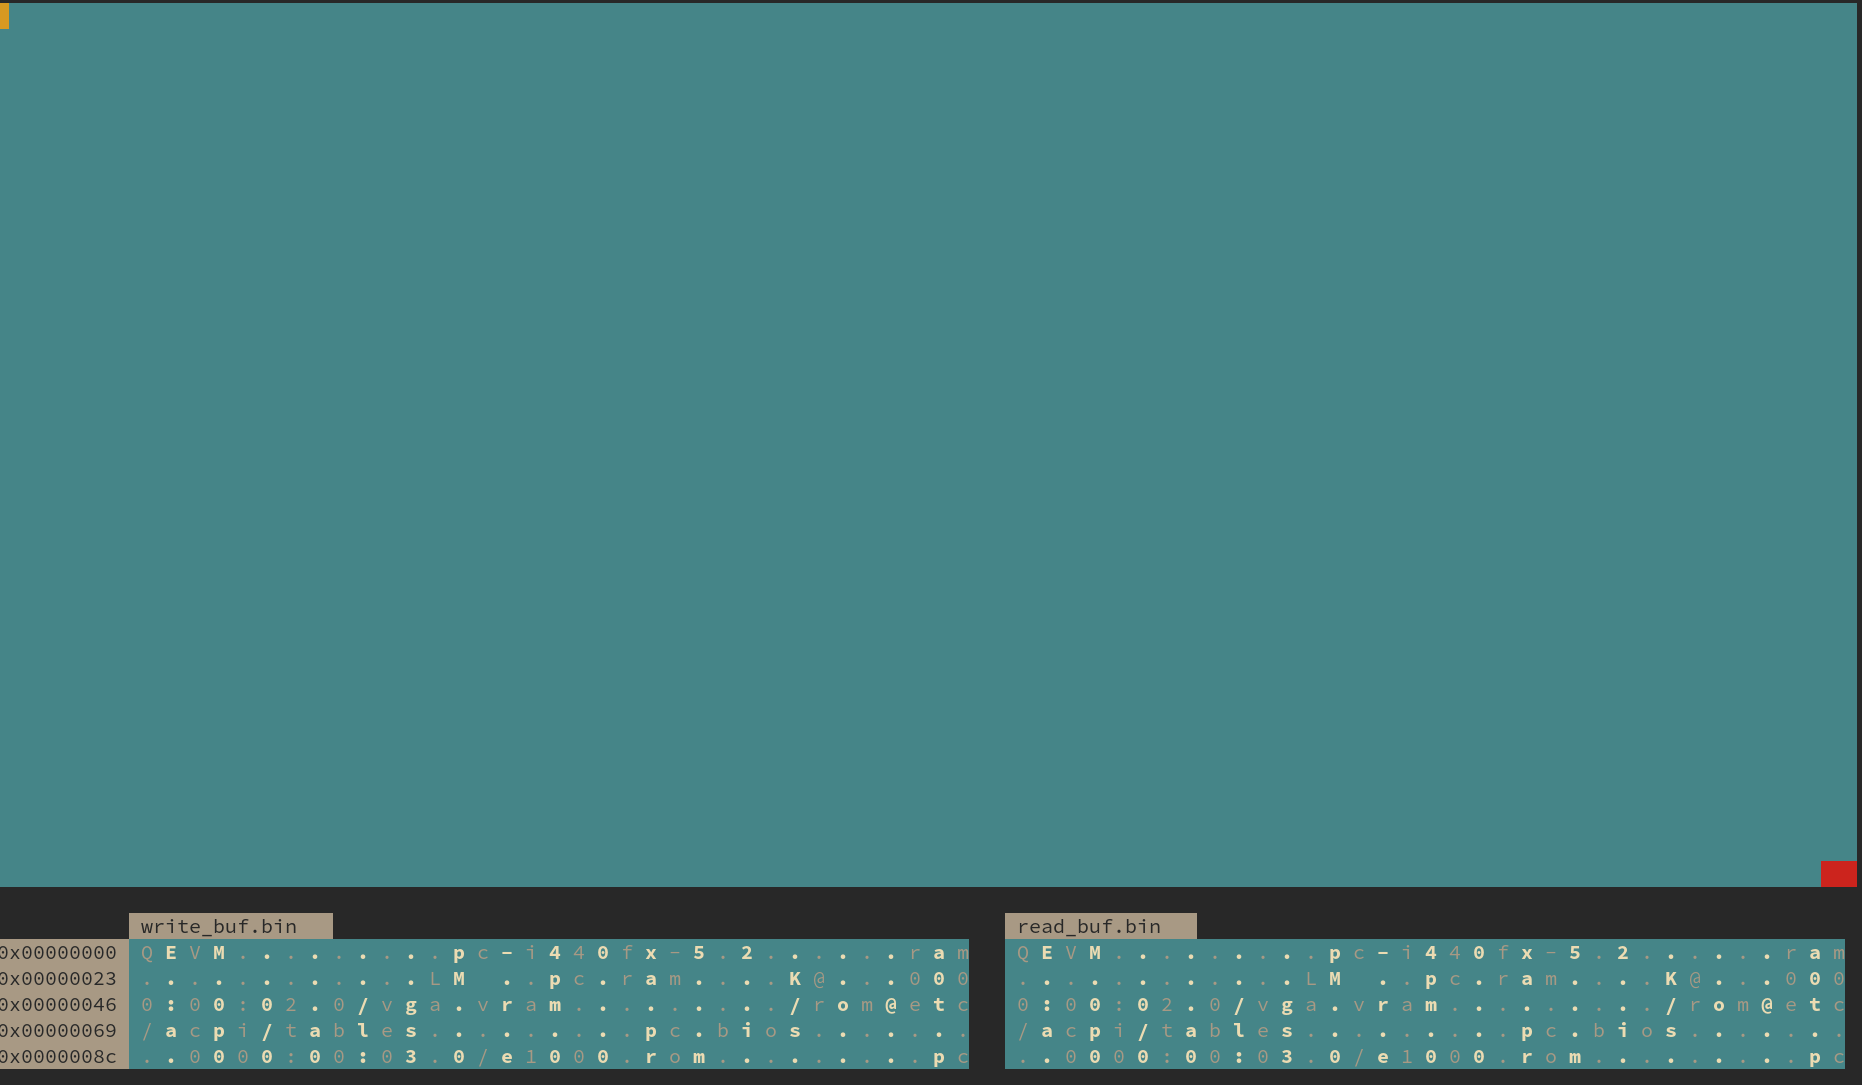
\includegraphics[scale=0.2]{include/haxcompare.png}
\caption{Représentation graphique d'un diff entre les données envoyées et reçues.}
\end{figure}


Dans un second temps, on a utilisé des outils d'analyse de paquets (wireshark), afin de récupérer les données associées aux paquets envoyés et ceux reçus (payloads).
Après la récupération des payloads nous avons procédé à une comparaison entre les paquets envoyés et reçus.




Nous avons remarqué que certains périphériques mappaient directement la mémoire de l'utilisateur sur le flux réseau de la migration.
Il existait une fenêtre de temps entre le moment où les données étaient écrites sur le fichier et le moment où les données étaient envoyées sur le flux réseau.
Étant donné que la zone mémoire en question n'est pas protégée par un mutex, l'utilisateur pouvait modifier cette zone mémoire en plein transfert.
Cela engendrait des différences entre les fichiers générés côté source et destination.


Après que le contenu des deux fichiers était équivalent, nous avons modifié l'algorithme pour générer un hash des données au lieu de les écrire dans un fichier.